%# -*- coding: utf-8-unix -*-

\chapter{机票数据分析及基线机票推荐算法}
\label{chap:baseline}
本章对研究用到的机票数据进行简要介绍及内容属性分析。在此分析的基础上,
给出用户偏好模型的表示方法并根据用户的偏好进行机票个性化推荐。
根据实验结果评估推荐算法的效果。本章的算法作为一个基线算法,是后续章节算法改进的基础与对照。

\section{数据来源及描述}
本论文研究工作使用的数据由国内知名的在线票务服务商提供。数据以表的格式组织,每条数据为一张机票订单。原始数据记录中的主要字段如表\ref{tab:fields}所示。
表格的前两项分别标识了唯一的订单以及对应的订票用户;由于国内部分城市有两个或更多个机场,所以需要标注航班的起飞机场和到达机场;舱位等级主要包括头等舱,商务舱和经济舱三个大类;飞机型号包含了飞机的大小等特征。

\begin{table}[!hpb]
  \centering
  \bicaption[tab:fields]{字段介绍}{原始机票订单数据的字段}{Table}{Fields of 
  Flight Data}
  \begin{tabular}{|c|c|} \hline 
    字段名称 & 字段描述\\ \hline
    Order Id & 订单ID \\ \hline
    User Id &  账户ID \\ \hline
    Order Date & 用户订票日期 \\ \hline
    Order Time & 用户订票时间 \\ \hline
    Takeoff Date & 起飞日期 \\ \hline
    Takeoff Time & 起飞时间 \\ \hline
    Departure City & 起飞城市 \\ \hline
    Arrival City & 落地城市 \\ \hline
    Airline & 航班所属航空公司 \\ \hline
    Departure Port & 起飞机场 \\ \hline
    Arrival Port & 到达机场 \\ \hline
    Class & 舱位等级 \\ \hline
    Price & 机票价格 \\ \hline
    Ticket Policy & 退、改签政策 \\ \hline
    Craft Size & 飞机型号 \\ \hline
  \end{tabular}
\end{table}

表格中的字段表明了机票数据高度结构化的特性。机票数据的属性与书籍、电影、音乐等物品的属性不同。后者的属性通常仅作为物品分类的依据,不能直接反映物品本身的内容。而机票数据的属性则可以代表机票本身的内容,进而直接影响用户的购买决策。另外,不同于上述物品固定的静态属性,机票的价格属于动态属性,即使对于相同航班的同一等级的舱位,其票价在起飞前会发生持续变动,并且变动的幅度很大。而价格作为机票内容中相当重要的一项,会在很大程度上影响用户的选择。因此,即使两张机票具有相同的的航班号和舱位等级,如果它们的价格不同,我们也不能将其当作同一个物品;
也难以直接使用以 User-Item 矩阵表示的协同过滤类型的方法进行机票推荐。根据机票数据具备的上述特性,我们主要使用基于内容的方法进行机票推荐。
此外,用户搜索时产出的候选机票数量约为一百左右,远低于传统推荐系统中成千上万的物品数量,但是每项候选机票都算作一个新的物品。机票个性化推荐相当于将这数百项候选机票按照用户的偏好进行个性化排序,并按照排序后的结果向用户展示。因此,我们首先需要为每位用户建立偏好模型。

\section{用户偏好模型构建}

用户在决策购买机票时,可能会受很多因素的影响。有些用户属于价格敏感类型,倾向于选择价格较低的机票;有些用户可能因公出差,而公司和某些航空公司有合作关系,航空公司就是这类用户的首要考虑因素;起飞时间、出发机场等属性则是和用户的个人行程安排相关。在构建用户偏好模型时,我们着重关注直接反应机票内容的特征属性。

\subsection{机票数据预处理与特征选取}

从表\ref{tab:fields}中可以发现,机票的特征主要分为两种类型。一种是包括机票价格、起飞时间的连续型特征,而其余的均为离散型特征。为了便于构建模型,我们将两个连续特征进行离散化。起飞时间的离散化过程比较直观,可以将时间分为上午、下午、傍晚、夜间等几个区间。而价格特征的离散化较为复杂。首先,不同航线具有不同的基准价格;其次,对于同一条航线,在距离起飞日期不同的天数,同一个价格可能代表不同的价位相对高低程度。结合实际的推荐应用场景,我们使用了如下公式作为价格指数:\\
\begin{equation}
	P_{KPI} = \frac{P_{std} - P_{cur}}{P_{std} - P_{low}}
\end{equation}\par
其中,$P_{std}$的含义是经济舱无折扣价格,是航空公司制定的标准价,变动频率很小(通常以年为单位);
$P_{cur}$是当前机票的价格,在每条订单记录中可以获取。$P_{low}$是本次搜索页面中的最低价。
从几项参数的含义可以看出,如果用户选择的机票价格很低,分子越大,等式的值越接近于1;反之,等式的值越小,当用户选择的票价高于经济舱全价时,价格指数的值小于0。因此,价格指数越大,代表用户对票价越敏感;反之亦然。我们可以使用价格指数代表多变而重要的价格特征。并且,通过该公式计算出的价格指数与航线、距离起飞日期天数等因素无关,进而具有良好的通用性。得到价格指数后,可以结合业务领域知识将其划分为数个有代表性的区间。\par
完成对连续型特征的离散化后,我们又选取了起飞机场、到达机场(对于包含多机场城市的航线)、航空公司、舱位等级、退改签政策、飞机型号等关键特征。这些特征可以初步理解为对机票内容的概括。至此,机票的一个特征可以表示为一个向量,该向量的每个维度代表该特征对应的每个可能的取值(区间);用户对一个特征中某个维度的偏好值可以由用户在对应维度所占的选择频数百分比来描述,选择频数可以通过用户的历史订单统计。由定义可知,用户在一个特征上所有维度的偏好值之和为1。\\

\begin{equation}
\label{eq:dict}
	\mathbf{p_f} = [alternative:frequency,\dots]
\end{equation}
\begin{equation}
\label{eq:pref}
	\mathbf{P_u} = [\mathbf{p_0},\mathbf{p_1},\dots,\mathbf{p_{|f|}}]
\end{equation}\par
式\ref{eq:dict}描述了用户在一个特征上的偏好。$\mathbf{p_f}$中的每个键值对代表了特征可能的取值及该用户选择的频数百分比。
式\ref{eq:pref}描述了用户的机票偏好模型。机票共有$|f|$个特征。$\mathbf{P_u}$中的每个向量代表了用户在机票各个特征的偏好情况。
考虑到不同的用户可能侧重于不同的特征,在得到机票的主要特征和用户的偏好表示模型后,
还需要为每个特征赋予权重。

\subsection{机票特征权重的计算}

特征的权重代表了该特征对用户的重要程度。通常,在用户更侧重的特征上,用户的偏好会更加集中。我们使用信息熵todo:cite来描述用户偏好的集中程度。信息熵的公式如下:
\begin{equation}
	H(\mathbf{X}) = E[-\ln (P(X))] = - \sum_{i=1}^n P(x_i)\ln P(X_i)
\end{equation}\par

上式的含义是特征$X$所包含的信息丰富程度,$x_i$是$X$中每个维度的取值。
注意,当某个维度的值为$0$时,根据极限定理,$0 \times \ln 0 = 0$
当取值越集中,即用户的偏好越集中时,信息熵的值越小。当熵值达到的最小值$0$时,表明用户的偏好都集中在一个维度;反之,如果用户的偏好越分散,则熵值越大。
当每个维度的取值相等时,熵达到最大值$\ln n$,$n$为特征的维度数目。
因此,信息熵具有的性质可以用来计算用户对于每个属性的偏好程度。为了消除特征维度的差异对熵值
带来的影响,我们对信息熵进行归一化处理:
\begin{equation}
  \overline{H}(\mathbf{f}) = \frac{H(\mathbf{f})}{\ln n}
\end{equation}
\begin{equation}
  W(f) = \frac{1 - \overline{H}(\mathbf{f})}{\sum_{f \in F}(1 - \overline{H}(\mathbf{f}))}
\end{equation}\par
$F$为机票的特征集合,$W(f)$为目标用户在特征$f$上的偏好权重。用户在每个特征的偏好与所有特征权重构成了完整的用户偏好模型。结合由搜索产生的候选机票列表,就可以为用户进行机票个性化推荐。

\section{基于用户偏好的机票个性化推荐算法}
\label{sec:base_rec}

前文提到,机票个性化推荐相当于将所有候选机票按照与用户的偏好的契合度评分进行排序。因此还需要定义根据用户偏好计算候选机票评分的方法。我们将机票表示为在每个特征的取值的集合。
\begin{equation}
  \mathbf{f} = [0,\dots,1,\dots,0]
\end{equation}
\begin{equation}
  \mathbf{T} = [\mathbf{f_0},\mathbf{f_1},\dots]
\end{equation}\par
列向量$\mathbf{f}$代表机票的一个特征,机票在该特征的取值对应的维度置1,其余维度均置0。 $\mathbf{T}$代表一张机票,是所有特征的集合。
\begin{equation}
	\label{eq:score}
	S = \sum_{f \in F}W_f*T_f^T*P_f
\end{equation}\par
根据机票的表示方法,我们可以计算每张候选机票的评分。式\ref{eq:score}描述了评分计算过程,
其含义是机票在每个特征的取值与用户偏好的契合度的加权之和。$W_f$是每个特征的权重;$T_f$是机票在该特征上的取值;$P_f$是该用户在该特征下的偏好向量。将搜索结果中的候选机票根据评分
进行重新排序就得到了针对该用户的个性化推荐结果。我们可以给出如下推荐算法:\par

\begin{algorithm}
\caption{基于用户偏好的机票推荐算法及应用}
\label{algo:pref_rec}
\begin{algorithmic}[1]
\Require
\Statex 用户历史订单 $O$
\Statex 机票特征集合 $F$
\Statex 搜索结果列表 $C$

\Ensure 排序后的机票列表 $R$

\State $P \gets extractPref(O,F)$;
\State $W \gets getPrefWeight(O,F)$;
\State $R \gets \emptyset$;
\For { $t \in C$}
\State $S_t \gets 0$
\For { $f \in F$}
\State $S_f += \frac{P[f][t_f]}{Sum(P[f])} \times W[f] $
\EndFor
\State Append $S_f$ to R
\EndFor 
\State Sort $R$ by score;
\State \Return $R$;
\end{algorithmic}
\end{algorithm}


\begin{algorithm}
\caption{用户偏好模型计算}
\label{algo:pref_cal}
\begin{algorithmic}[1]
\Require
\Statex 用户历史订单 $O$
\Statex 机票特征集合 $F$
\Ensure
\Statex 用户的偏好模型 $P$

\Function {extractPref}{$O, F$}
\State $P \gets \emptyset$;
\For{$order \in O$}
\For{$f \in F$}
\State $P[f][order_f] += 1$;
\EndFor	
\EndFor 
\State \Return $P$;
\EndFunction

\Function {getPrefWeight}{$P$}
\State $W \gets \emptyset$
\For{$p_f \in P$}
\State $\overline{H}(\mathbf{p_f}) \gets \frac{H(\mathbf{p_f})}{\ln |p_f|}$
\EndFor
\For{$p_f \in P$}
\State $W_f \gets \frac{1 - \overline{H}(\mathbf{p_f})}{\sum_{f \in F}(1 - \overline{H}(\mathbf{p_f}))}$
\EndFor
\State \Return $W$
\EndFunction

\end{algorithmic}
\end{algorithm}\par

算法\ref{algo:pref_rec}是机票个性化推荐的整体流程。首先获取每个用户的偏好模型,再对搜索结果
中的每条候选机票计算评分并排序。以$C$代表机票搜索结果,$O$代表用户的历史订单,则算法复杂度是$O(|O|*|C|*\log|C|)$。其中,$|C|*\log|C|$是计算评分并排序的时间复杂度。
我们可以离线计算并存储用户的偏好模型,包括特征偏好及特征权重,见算法\ref{algo:pref_cal}。
那么实际使用场景中的推荐服务时间复杂度仅为$O(|C|*\log|C|)$,只与候选航班数量相关。
因此,算法已经具备在生产环境上使用的条件。\par
在生产环境的部署阶段,我们首先进行一次全量的用户偏好模型计算,将用户模型结构化后存储在Redis中,
并封装成对外数据接口。随后,还会对模型进行增量更新,每天会抽取出前一天提交过订单的用户,为这部分用户更新偏好。因此,模型后续维护的成本很小。当接受用户查询时,搜索引擎在检索候选机票的同时向数据接口发送请求以获取用户的偏好模型。相比于上百项搜索结果,拉取偏好模型的负载带来的影响很小,不影响用户体验。我们在前端计算每张机票的评分,并按照评分由高向低的顺序进行展示,可以灵活控制算法模型。\par

\section{数据实验与结果分析}

\subsection{数据分布与统计}
本节我们对推荐结果进行验证与分析。我们使用2013年1月至2015年7月的国内机票订单数据进行实验。该数据集包含了国内全部航线的直飞机票订单。有些航线如北京-上海较为热门,每天有大量旅客往返。航班也很密集;而大部分航线的航班数量都不是很多,属于非热门航班。机票订单数据呈长尾分布。考虑到机票个性化推荐算法的实际应用场景,我们这里多采用较热门的航线,因为只有这类航线才有较多的候选机票列表。

\begin{figure}
\centering
\subfigure[航线订单数量图]{
 \label{fig:total_order}
 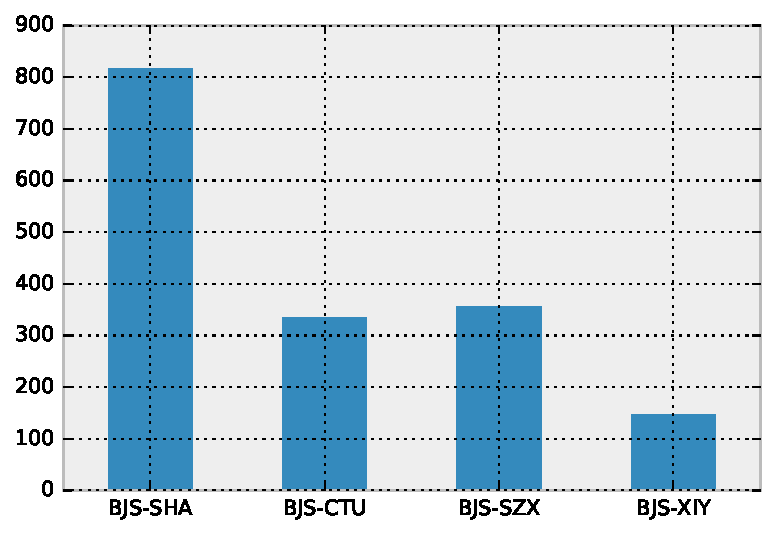
\includegraphics[width=0.49\linewidth]{03/1_total_order.pdf}}
\subfigure[航线用户数量图]{
 \label{fig:total_user}
 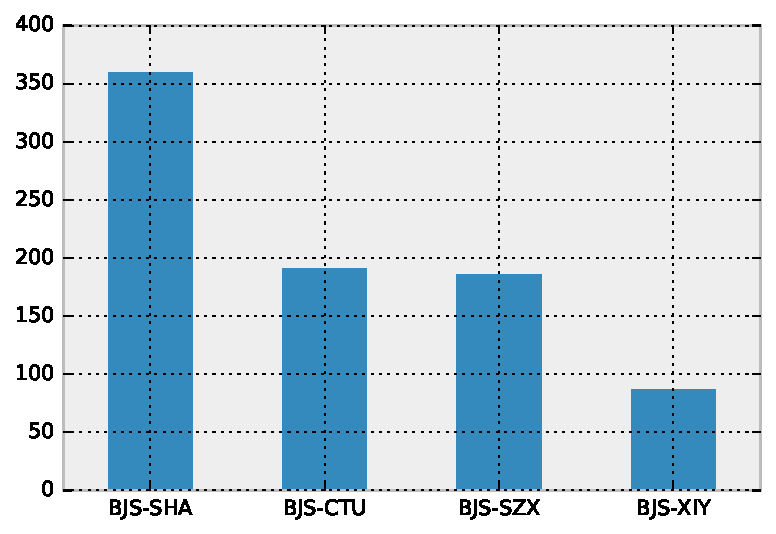
\includegraphics[width=0.49\linewidth]{03/2_total_user.pdf}}
\bicaption[fig:total]{数据统计}{测试航线总体数据统计}{Fig}{Figure for Data Statistic in Test Alrlines}
\end{figure}\par

我们选取了北京到上海(BJS-SHA),北京到成都(BJS-CTU),北京到深圳(BJS-SZX),北京到西安(BJS-XIY)这四条航线作为测试航线。图\ref{fig:total_order}为测试航线的航班数量分布图,其横轴分别代表四条航线,纵轴代表对应航线上航班总量(单位:千条)。
图\ref{fig:total_user}为测试航线上用户数量分布图,其纵轴代表对应航线上用户总数(单位:千人)。通过上面两图我们可以发现,这四条航线的订单数量和乘客数量都很大,在国内具有很高的热门度。其中北京到上海这条航线的热门程度最高,其订单数量和用户数量都远多于其他三条。其中北京到上海和北京到深圳这两条航线的订单、用户数量比达到$2.0$以上;北京到成都和北京到西安的订单、用户数量比只有$1.6$左右,表明后两条航线上的新用户数量远多于前者。我们认为这可以在一定程度上反应城市的性质。往返于北京-上海和北京-深圳的旅客可能更多是出于商务办公目的,因此会造成多次往返的行为;而往返于北京-成都和北京-西安的旅客则更可能是出于休闲旅游目的。\par

\begin{figure}
\centering
\subfigure[用户数量百分比]{
 \label{fig:user_user_percent}
 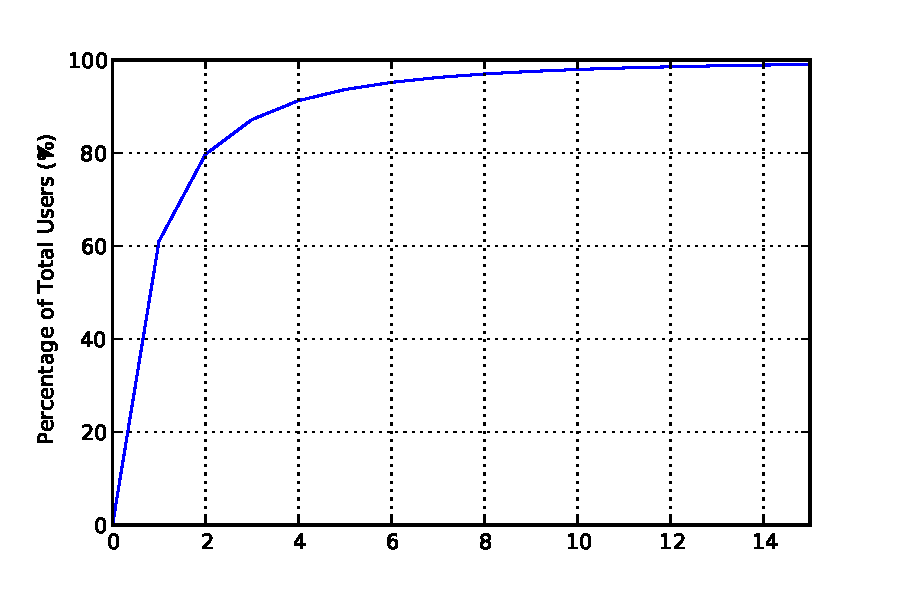
\includegraphics[width=0.49\linewidth]{03/3_user_of_user-count.pdf}}
\subfigure[用户-订单数量百分比]{
 \label{fig:user_order_percent}
 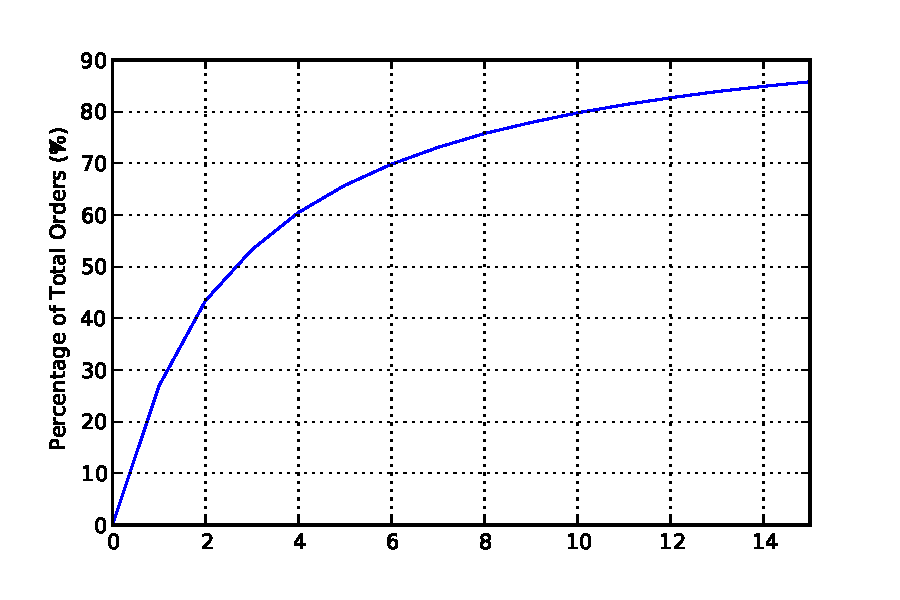
\includegraphics[width=0.49\linewidth]{03/4_user_of_order-count.pdf}}
\bicaption[fig:total]{分布统计}{北京-上海订单、用户分布统计}{Fig}{Figure for Data Statistic in Test Alrlines}
\end{figure}\par

我们针对北京-上海航线做了详细的数据分布统计。图\ref{fig:user_user_percent}展示了该航线的用户订单数与用户数量的分布关系,其横轴代表数据集用户的订单数,纵轴代表当前用户数占总用户总数的百分比。结合图表,其含义是订单数量不超过1单的用户占用户总数量的$61\%$;订单数量不超过2单的用户占总量的80\%;99\%以上的用户订单数量在10以下。图\ref{fig:user_order_percent}展示了该航线用户订单数与订单总数量之间的分布关系,其纵轴代表当前订单数占订单总数的百分比。虽然订单数为1单的用户占总用户数的$61\%$,但仅占了$25\%$的订单;订单数量不超过$15\%$的用户占了总订单量的$85\%$。订单数量过多的用户很可能是旅行社代理、部门秘书等代订用户,这部分用户通常为多个乘机人订票,因此从他们的历史订单学习到的偏好几乎不具有代表性,并且代订用户的出行往往有极强的计划性,因此为其进行推荐的效果有限。结合用户数量和订单的分布情况,我们将订单数量多于15的用户从实验数据集中剔除;由于没有测试数据,订单数量为1单的用户也不能用于实验。

\par todo:介绍模拟搜索结果

\subsection{推荐效果评价指标}
为了评估基于偏好模型的算法是否能够精准挑选出适合用户的航班,我们需要引入对推荐效果的评价考核指标。机票推荐属于隐式推荐,用户几乎没有对机票进行主动评分、评价等反馈。根据前文介绍,我们也不能简单的将相同航班、相同舱位的机票当作同一个物品。因此反馈也不具备很强的参考价值。同时,结合业务场景,机票搜索引擎每次向用户展示几十到上百条候选机票,用户往往只会选定一个航班进行下单,是一种只具备隐式正反馈的场景,并且正样本的比例极低。我们构建的用户偏好模型也是建立在假定用户对当次选购的机票具有最高的偏好度的基础上。balabala我先回去了。



\label{sec:base_rec}



todo:figure of entropy.
todo:figure of result.